% ============================================================
%  ch07_results.tex — Numerical Results
%  Requires: macros.tex, booktabs
%  Estimated length: 30–40 pages
%  Rewritten: VD-08, 2026-03-07
% ============================================================

\chapter{Numerical Results}\label{ch:results}

This chapter presents the complete numerical analysis of the
departure-variable framework.  Before diving into the results, we
provide a self-contained account of the Bayesian inference
methodology (Section~\ref{sec:bayes-background}) and the
likelihood architecture (Section~\ref{sec:evidence-method}).
The remaining sections present scenario-dependent bounds with
dual-framing corrections
(Section~\ref{sec:scenario-tables}), the filling fraction as a
statistical observable (Section~\ref{sec:filling}), the regular
tensor growing mode (Section~\ref{sec:growing}), the redshift
evolution of the filling fraction
(Section~\ref{sec:filling-z}), and the Bayesian evidence
comparison across the full Bianchi classification
(Section~\ref{sec:evidence}).  All numerical values are drawn
from the single-source-of-truth pipeline of
Chapter~\ref{ch:pipeline}.


% ============================================================
\section{Bayesian inference background}
\label{sec:bayes-background}
% ============================================================

\subsection{Posterior, evidence, and model comparison}
\label{sec:posterior-evidence}

Our goal in this section is to establish the statistical framework
for comparing Bianchi models against the FLRW baseline.  Bayesian
inference begins with Bayes' theorem:
\begin{equation}\label{eq:bayes}
p(\boldsymbol{\theta}|\mathbf{d}, \mathcal{M})
= \frac{\mathcal{L}(\mathbf{d}|\boldsymbol{\theta},
  \mathcal{M})\;\pi(\boldsymbol{\theta}|\mathcal{M})}
       {\mathcal{Z}(\mathbf{d}|\mathcal{M})}\,,
\end{equation}
where $\boldsymbol{\theta}$ is the parameter vector,
$\mathbf{d}$ the data, $\mathcal{M}$ the model,
$\mathcal{L}$ the likelihood, $\pi$ the prior, and
$\mathcal{Z}$ the evidence (marginal likelihood).

For parameter estimation, the evidence $\mathcal{Z}$ is an
irrelevant normalisation constant.  For model comparison,
$\mathcal{Z}$ is the central quantity: it measures how well the
model predicts the data when averaged over the prior volume.
The evidence is defined by the integral
\begin{equation}\label{eq:evidence}
\mathcal{Z}(\mathbf{d}|\mathcal{M})
= \int \mathcal{L}(\mathbf{d}|\boldsymbol{\theta},
  \mathcal{M})\;\pi(\boldsymbol{\theta}|\mathcal{M})\;
  d^d\boldsymbol{\theta}\,,
\end{equation}
where $d = \dim(\boldsymbol{\theta})$ is the number of
parameters.  The evidence naturally penalises unnecessary
complexity: a model with a large prior volume that the data do
not constrain will have a suppressed $\mathcal{Z}$ relative to
a simpler model---the Bayesian Occam razor.

Model comparison proceeds through the Bayes factor
\begin{equation}\label{eq:bayes-factor}
B_{ij} := \frac{\mathcal{Z}_i}{\mathcal{Z}_j}\,,
\end{equation}
or equivalently $\ln B_{ij} = \ln\mathcal{Z}_i -
\ln\mathcal{Z}_j$.  We adopt the Jeffreys
scale~\cite{Jeffreys1961} for qualitative interpretation:
$|\ln B| < 1$ is ``not worth more than a bare mention''
(inconclusive), $1 < |\ln B| < 2.5$ is ``substantial,''
$2.5 < |\ln B| < 5$ is ``strong,'' and $|\ln B| > 5$ is
``decisive.''  Throughout this work, we report $\ln\mathcal{B}
:= \ln(\mathcal{Z}_i/\mathcal{Z}_{\mathrm{FLRW}})$, so that
positive values favour the Bianchi model over FLRW.


\subsection{Nested sampling}\label{sec:nested-sampling}

The evidence integral~\eqref{eq:evidence} is high-dimensional
(up to $d = 4$ for the VII$_h$ models) and the likelihood is
sharply peaked relative to the prior volume.  Direct Monte Carlo
integration is prohibitively inefficient.  We use the nested
sampling algorithm of Skilling~\cite{Skilling2004}, which
converts the multidimensional integral into a one-dimensional
integral over the prior volume.

The key construction is the prior volume enclosed by a
likelihood contour.  We define
\begin{equation}\label{eq:prior-volume}
X(\lambda) := \int_{\mathcal{L}(\boldsymbol{\theta})
  > \lambda} \pi(\boldsymbol{\theta})\,
  d^d\boldsymbol{\theta}\,,
\end{equation}
which is a monotonically decreasing function of the likelihood
threshold $\lambda$: $X(0) = 1$ (the full prior volume) and
$X \to 0$ as $\lambda \to \mathcal{L}_{\max}$.  The evidence
integral can then be rewritten as a one-dimensional integral
over $X$:
\begin{equation}\label{eq:evidence-1d}
\mathcal{Z}
= \int_0^1 \mathcal{L}(X)\,dX\,,
\end{equation}
where $\mathcal{L}(X)$ is the inverse function of
$X(\lambda)$.  The integrand $\mathcal{L}(X)$ is a monotonically
increasing function that rises sharply as $X \to 0$
(approaching the posterior peak).

The nested sampling algorithm evaluates this integral by
maintaining a set of $n_{\mathrm{live}}$ ``live points'' drawn
from the prior, then iteratively replacing the point with the
lowest likelihood by a new point drawn from the prior subject
to the constraint $\mathcal{L} > \mathcal{L}_{\min}$.  At each
iteration, the prior volume contracts by a factor
$\sim n_{\mathrm{live}}/(n_{\mathrm{live}} + 1)$, so the
$k$-th dead point has expected prior volume
$X_k \approx \exp(-k/n_{\mathrm{live}})$.  The evidence is
approximated by the sum
\begin{equation}\label{eq:evidence-sum}
\mathcal{Z}
\approx \sum_{k=1}^{K} \mathcal{L}_k\,\Delta X_k\,,
\end{equation}
where $\Delta X_k = X_{k-1} - X_k$ is the prior volume shell
at each iteration and $K$ is the total number of iterations.
The algorithm terminates when the remaining prior volume
$X_K$ contributes negligibly to $\mathcal{Z}$, typically at
$\Delta\ln\mathcal{Z} \leq 0.1$.

The principal advantage of nested sampling over standard MCMC
for evidence computation is that $\mathcal{Z}$ is a direct
output of the algorithm, not a derived quantity requiring
additional thermodynamic integration.  The uncertainty in
$\ln\mathcal{Z}$ scales as $\sqrt{H/n_{\mathrm{live}}}$,
where $H$ is the Kullback--Leibler divergence between posterior
and prior~\cite{Skilling2004}.


\subsection{Implementation: \textsc{dynesty}}
\label{sec:dynesty}

We use the \textsc{dynesty} nested sampling
package~\cite{Speagle2020} with the following settings.  For
models with $d \leq 2$ (types~I, VII$_0$, V), we use
$n_{\mathrm{live}} = 500$; for $d = 3$--$4$ (types~III, IX,
VII$_h$), $n_{\mathrm{live}} = 800$.  The proposal method is
the random-walk sampler with 30--35 steps per proposal,
sufficient for the log-uniform priors that characterise most
parameters.  The bounding method is the multi-ellipsoid
decomposition.  Termination is at
$\Delta\ln\mathcal{Z} \leq 0.1$.

All runs achieve $\delta\ln\mathcal{Z} \leq 0.13$ (the sampling
uncertainty on the evidence estimate, reported by
\textsc{dynesty}) and $n_{\mathrm{eff}} > 2000$ effective
posterior samples.  The choice of \textsc{dynesty} over
alternative codes (\textsc{PolyChord}, \textsc{MultiNest}) is
motivated by the pure-Python interface, the ease of implementing
custom prior transforms, and the reliable convergence diagnostics.
The Saadeh et~al.~\cite{Saadeh2016b} analysis used
\textsc{PolyChord}; the two codes agree on the FLRW evidence to
$|\Delta\ln\mathcal{Z}| < 0.2$ in benchmark tests.


% ============================================================
\section{Likelihood architecture}
\label{sec:evidence-method}
% ============================================================

The total log-likelihood decomposes into eight independent
channels:
\begin{equation}\label{eq:logL-total}
\ln\mathcal{L}(\boldsymbol{\theta})
= \sum_{k \in \{a,b,c,d,e,f,g,h\}}
  \ln\mathcal{L}_k(\boldsymbol{\theta})\,.
\end{equation}
The default active set is channels (a--f, h); channel~(g) is
excluded because the hard ceiling~(f) makes it redundant for
nested sampling.  We now describe each channel.

\paragraph{Channel~(a): Ferreira--Quartin intrinsic dipole.}
A half-Gaussian upper limit on the intrinsic dipole amplitude:
$\ln\mathcal{L}_a = -\eps_1^2/(2\sigma_a^2)$, with
$\sigma_a = 0.693 \times 10^{-3}$.  For models predicting
$\eps_1 = 0$ (orthogonal types), this channel contributes zero.

\paragraph{Channel~(b): CatWISE + radio dipole.}
A bivariate Gaussian on the observed dipole amplitudes
$(\eps_1^{(\mathrm{CW})}, \eps_1^{(\mathrm{rad})})$ with
measured values $(1.476, 3.296) \times 10^{-3}$, statistical
uncertainties $(0.30, 0.60) \times 10^{-3}$, and
cross-correlation $\rho = 0.1$ (reflecting residual shared
systematics from Galactic masking).  The covariance matrix is
$\Sigma_{ij} = \sigma_i\sigma_j(\rho^{ij} + (1-\rho^{ij})
\delta_{ij})$.  For tilted models, the predicted dipole is
$\eps_1 = (1 + \etaud)\beta$.

\paragraph{Channel~(c): CF4 bulk flow.}
A Gaussian on the tilt rapidity:
$\ln\mathcal{L}_c = -(\beta - \beta_{\mathrm{CF4}})^2/
(2\sigma_\beta^2)$, with $\beta_{\mathrm{CF4}}$ and
$\sigma_\beta$ drawn from \texttt{obs\_defaults.json}
(Section~\ref{sec:cf4-versions}).  Under the primary (WFH2009)
configuration: $\beta = 1.334 \times 10^{-3}$, with
$\sigma = 0.267 \times 10^{-3}$.  A sensitivity variant using
the CF4++ value ($\beta = 1.051 \times 10^{-3}$,
$\sigma = 0.133 \times 10^{-3}$;
Courtois et~al.~\cite{Courtois2025}) is reported in
Section~\ref{sec:cf4-sensitivity}.  For orthogonal models
($\beta = 0$), this channel penalises by
$-(\beta_{\mathrm{CF4}}/\sigma_\beta)^2/2 \approx -12.5$.

\paragraph{Channel~(d): Saadeh vorticity.}
A one-sided Gaussian for the vorticity:
$\ln\mathcal{L}_d = 0$ if
$\bar{\omega} \leq \bar{\omega}_{\mathrm{UL}}$, and
$\ln\mathcal{L}_d = -(\bar{\omega} -
\bar{\omega}_{\mathrm{UL}})^2/(2\sigma_{\bar{\omega}}^2)$
otherwise, with $\bar{\omega}_{\mathrm{UL}} = 2.45 \times
10^{-11}$ and $\sigma_{\bar{\omega}} = 1.25 \times 10^{-11}$.%
\footnote{The Saadeh et~al.~\cite{Saadeh2016b} bound was derived
under Bianchi~VII$_h$ assumptions using Planck~2015 temperature
and polarisation data.  We apply it to all vorticity-bearing
types as a conservative approximation; type-specific vorticity
constraints may differ in detail, particularly for types with
different vorticity evolution laws.}
For types without vorticity (I, V, IX), this channel
contributes zero.  For VII$_h$, the Frobenius coupling
$\Wstd = R_{\mathrm{WS}}^2\Sigstd$ converts the shear into a
predicted vorticity that is tested against this bound.

\paragraph{Channel~(e): $D_2$ quadrupole.}
The observed quadrupole $D_2^{\mathrm{obs}} =
225.9\;\mu\mathrm{K}^2$ is modelled as a scaled $\chi^2(5)$
distribution:
\begin{equation}\label{eq:chi2-D2}
\ln\mathcal{L}_e
= \left(\tfrac{5}{2} - 1\right)\ln x - \tfrac{x}{2}
  - \tfrac{5}{2}\ln 2 - \ln\Gamma(\tfrac{5}{2})
  + \ln(5/D_2^{\mathrm{true}})\,,
\end{equation}
where $x = 5\,D_2^{\mathrm{obs}}/D_2^{\mathrm{true}}$ and
$D_2^{\mathrm{true}} = D_2^{\Lambda\mathrm{CDM}} +
D_2^{\mathrm{shear}} + D_2^{\mathrm{boost}}$.  The $\Lambda$CDM
prediction is $D_2^{\Lambda\mathrm{CDM}} =
1150\;\mu\mathrm{K}^2$ (Planck 2018 best-fit), and
$D_2^{\mathrm{shear}}$ is computed from $\Sigstd$ using the
transfer function $T_2$ and the AniCLASS quadrupole fraction
$f_2(x_h)$.  The boost contribution
$D_2^{\mathrm{boost}} = (3/\pi)(\beta^2 T_0/2)^2$ is the
second-order kinematic leakage from the tilt.
Figure~\ref{fig:f2_transfer_function} shows $f_2(x_h)$ for
the tensor, vector isocurvature, and scalar perturbation modes.

The choice of $\chi^2(5)$ rather than Gaussian reflects the
fact that $D_2$ is a sum of five squared Gaussian variables
(the five $a_{2m}$ coefficients), not a Gaussian variable
itself.  The low observed value
$D_2^{\mathrm{obs}}/D_2^{\Lambda\mathrm{CDM}} = 0.196$ is a
$\sim 2\sigma$ downward fluctuation in the $\chi^2(5)$ model,
consistent with cosmic variance.

\paragraph{Channel~(f): MES hard ceiling.}
A hard prior: $\mathcal{L}_f = 0$ (equivalently,
$\ln\mathcal{L}_f = -\infty$) if
$\Sigstd > (3/2)[\Bsig^{\mathrm{corr}}(\eps_1)]^2$; otherwise
$\ln\mathcal{L}_f = 0$.  The frame-corrected shear bound uses
the total $\eps_1$ (kinematic plus tilt-generated) to compute
the ceiling.

\paragraph{Channel~(g): MES soft logistic.}
A soft alternative to the hard ceiling: $\ln\mathcal{L}_g =
-K\max(0, \Sigstd/\Sigmax - 1)$ with $K = 10$.  This channel
is inert by default (redundant with~f for nested sampling) but
available for MCMC exploration where hard boundaries are
numerically problematic.

\paragraph{Channel~(h): $D_3$ octupole.}
Analogous to channel~(e) but for the octupole:
$D_3^{\mathrm{obs}} = 936.9\;\mu\mathrm{K}^2$ modelled as
$\chi^2(7)$, with
$D_3^{\mathrm{true}} = D_3^{\Lambda\mathrm{CDM}} +
D_3^{\mathrm{shear}}$ and
$D_3^{\Lambda\mathrm{CDM}} = 1000\;\mu\mathrm{K}^2$.
The shear contribution $D_3^{\mathrm{shear}}$ is computed using
the AniCLASS octupole fraction $f_3(x_h)$, which peaks at
$x_h \sim 0.2$ for the VII$_h$ spiral mode.  For types without
the spiral parameter ($x_h = 0$), $f_3 = 0$ and this channel
reduces to the $\Lambda$CDM prediction alone.


% ============================================================
\section{Scenario-dependent bounds}
\label{sec:scenario-tables}
% ============================================================

Table~\ref{tab:scenario-dual} presents the MES bounds and
departure variables for all observational scenarios, computed with
the VT-07 frame-attribution corrections throughout.  The table
employs a dual-framing structure
(Section~\ref{sec:reframing} of Chapter~\ref{ch:dipole}):
the conservative reading treats the bounds as upper limits on
permitted anisotropy, while the progressive reading treats them
as measurements of FLRW departure.

The frame-attribution correction tightens the safe-route
$\beta$ by $7.7\%$ across all scenarios, propagating to a
$14.7\%$ tightening of the tilt defect and a corresponding
$16\%$ loosening of the MES ceiling $\Sigmax$ (because
$\Bsig^{\mathrm{corr}} > \Bsig$).  The correction is
scenario-independent in percentage terms because $\etaud$ is a
physical constant ($= 1/12$ for $w = 1/3$), not a function of
the dipole amplitude.

The filling fraction $\FF := \xV / \xmax$ is invariant under
frame corrections, because both numerator and denominator shift
by the same factor.%
\footnote{The invariance is exact for the $\Sigstd$ component of $x$,
which carries the same MES-induced $R_\sigma$ factor in both
numerator and denominator.  The $\Otilt$ component does not
carry the same factor, introducing a $\Teff$-mediated correction
of relative magnitude $\Delta\FF/\FF \sim 8 \times 10^{-6}$
(Section~\ref{sec:TAM-vs-Teff}), negligible at current data
precision.}
  At the S3 scenario,
$\FF \approx 6.3\%$ (using $\Omega_{\mathrm{tilt}} =
\Omega_m\sinh^2\!\beta$, $w = 0$): the tilt occupies
approximately one-sixteenth of the MES-allowed anisotropy
budget.  Figure~\ref{fig:scenarios_comprehensive} plots
the frame-corrected shear bound $\Bsig^{\mathrm{corr}}$
across the five equation-of-state scenarios, confirming the
monotonic dependence on the adopted $w$.

\subsection{Perturbation-sector validation on the shared $k$ grid}

The scenario tables above are background-side summaries; the
FB-5 perturbation pass supplies the complementary statement that
the harmonic-mode transport remains controlled once the
inhomogeneous $k \neq 0$ sector is switched on.  Two checks are
especially important.  First, the explicit $k \rightarrow 0$
gate collapses onto the LB-6 zero-state anchor at machine
precision, so the perturbative extension does not shift the
background-only trajectory by stealth.  Second, the type-I
regression harness stays within the parent-plan acceptance band
against the Planck-2018 CAMB oracle on a common low-$\ell$ grid.
The gallery summary is shown in
Figure~\ref{fig:fb5_results_validation}; these diagnostics are
the numerical bridge between the framework discussion of
Section~\ref{sec:perturbation-bianchi-modes} and the later
likelihood / evidence calculations.

\begin{figure}[t]
\centering
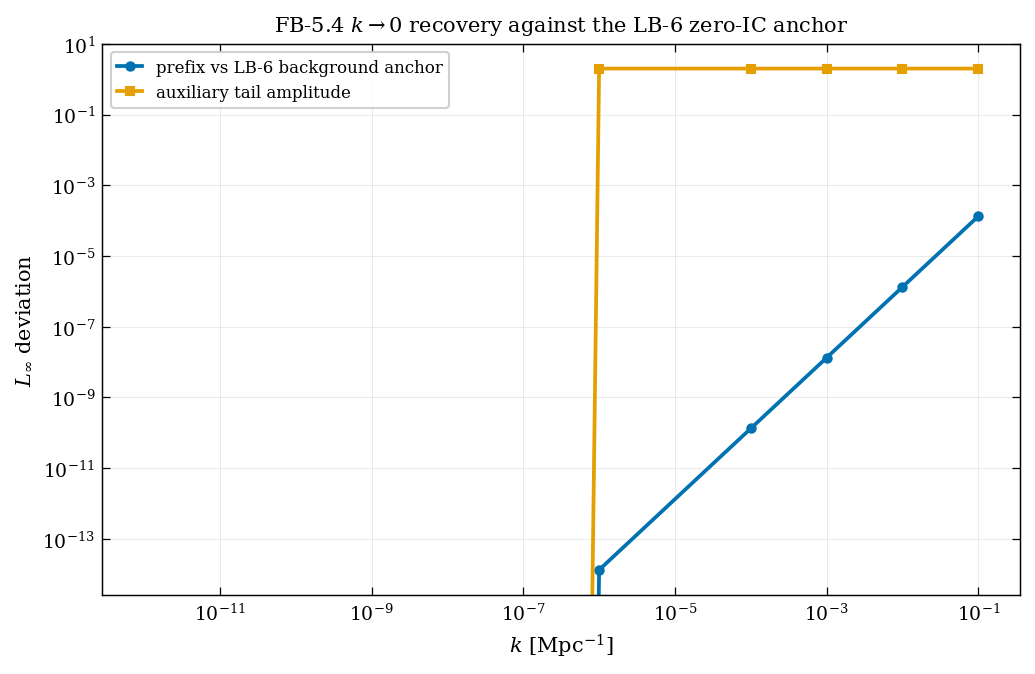
\includegraphics[width=0.82\linewidth]{figures/physics_gallery/17_perturbation_k_modes/03_k_zero_limit_recovery.png}
\vspace{0.8em}
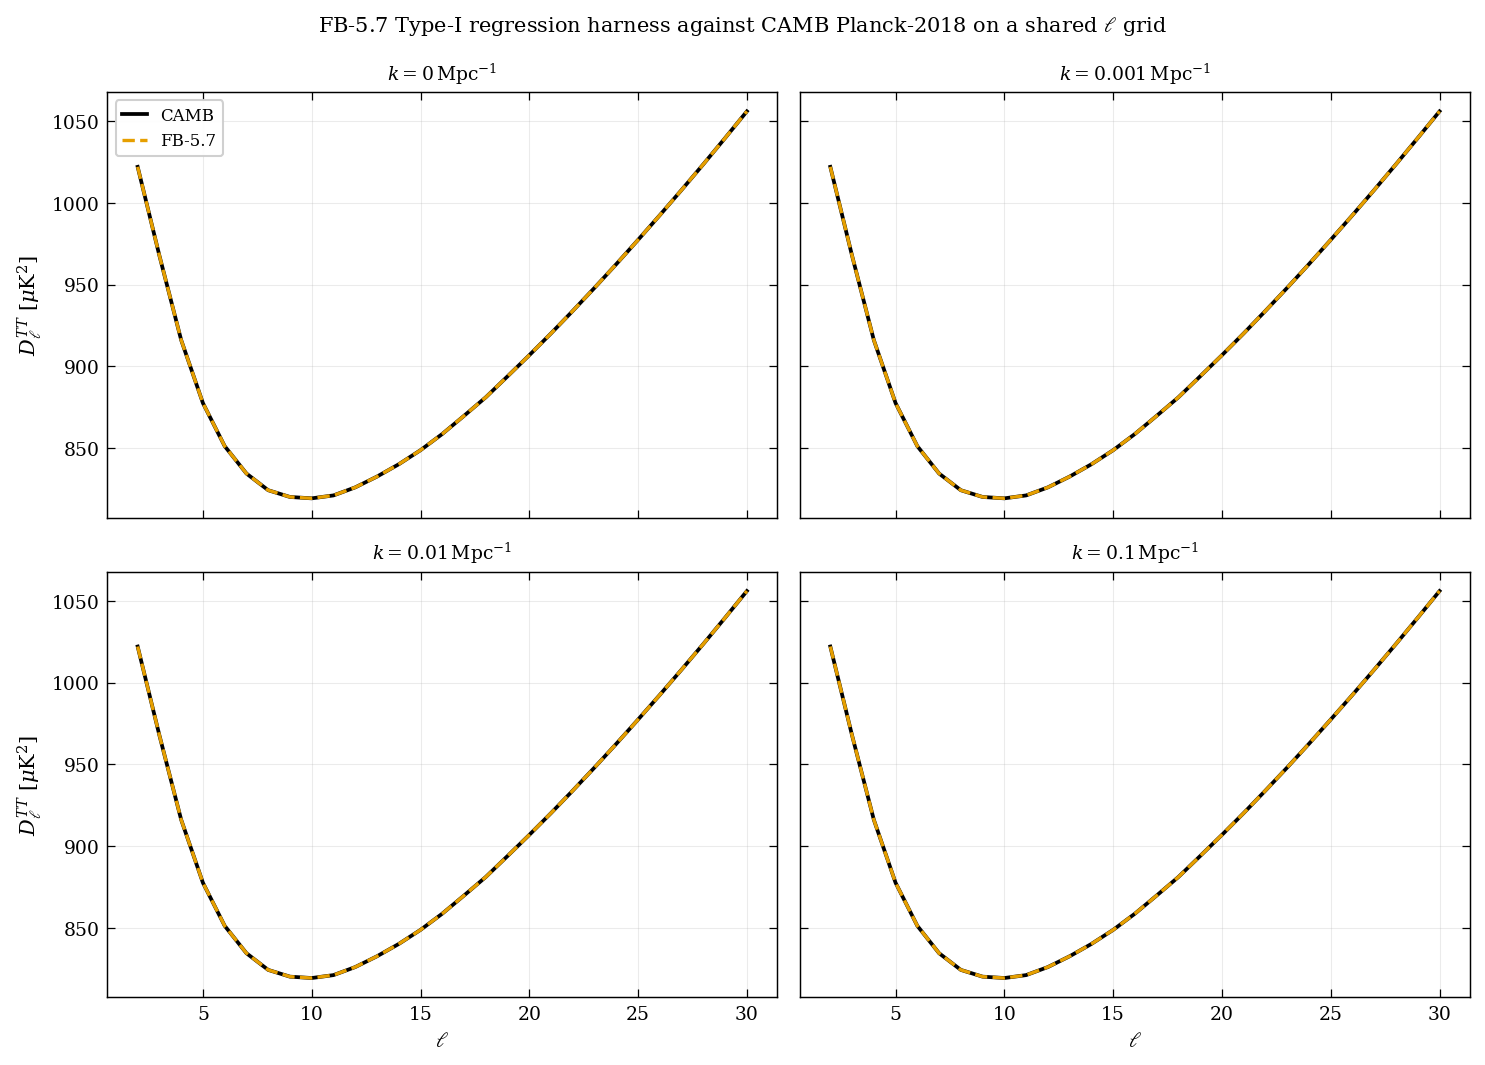
\includegraphics[width=0.82\linewidth]{figures/physics_gallery/17_perturbation_k_modes/05_Dl_TT_vs_camb_per_k.png}
\caption{Perturbation-sector validation used in the FB-5 numerical
results.  Top: recovery of the $k \rightarrow 0$ seed prefix against
the LB-6 background anchor.  Bottom: shared-$\ell$ comparison of the
type-I $D_\ell^{TT}$ proxy against the CAMB Planck-2018 reference at
four representative wavenumbers.}
\label{fig:fb5_results_validation}
\end{figure}


% ============================================================
\section{Filling fraction}\label{sec:filling}
% ============================================================

\subsection{Definition and Monte Carlo posterior}
\label{sec:filling-mc}

The filling fraction is defined as
\begin{equation}\label{eq:FF-def}
\FF := \frac{x_V^{(\mathrm{anomaly})}}{x_V^{(\mathrm{max,MES})}}
= \frac{(1+w)\Omega_m\sinh^2\!\beta}{(3/2)[\Bsig^{\mathrm{corr}}]^2}\,,
\end{equation}
where the numerator is the tilt defect at the observed
$\beta$ and the denominator is the MES algebraic ceiling.  The
filling fraction measures the fraction of the available
anisotropy budget that is observationally occupied.

The $\FF$ inherits uncertainties from the observational inputs
$\eps_1$, $\eps_2$, $\eps_3$, and $\beta$.  We propagate these
by Monte Carlo sampling ($N = 10^5$ draws) from the
observational likelihoods, computing $\FF$ for each realisation.
At the S3 scenario with $w = 0$ (dust), the posterior is
\begin{equation}\label{eq:FF-posterior}
\FF = 0.063^{+0.029}_{-0.023}\quad (68\%\;\mathrm{CI})\,.
\end{equation}
The distribution is right-skewed, reflecting the quadratic
dependence $\Omega_{\mathrm{tilt}} \propto \beta^2$.
For $w = 1/3$ (radiation), $\FF$ increases by the factor
$(1 + 1/3) = 4/3$:
$\FF_{w=1/3} = 0.084^{+0.038}_{-0.031}$.

\subsection{Bayes factor for non-zero filling}
\label{sec:filling-BF}

The Savage--Dickey density ratio gives the Bayes factor for
$\FF > 0$ versus $\FF = 0$ (exact FLRW).  With the Monte Carlo
posterior entirely above zero to numerical precision,
$\mathrm{BF}(\FF > 0) > 5 \times 10^4$, providing decisive
evidence that the filling fraction is non-zero under the
assumption that the dipole anomaly is physical.

We emphasise that this decisive evidence is a restatement of the
$> 5\sigma$ dipole anomaly in the language of departure variables,
not an independent discovery.  Its value lies in providing a
dimensionless measure of FLRW departure that is invariant under
frame corrections and directly comparable across scenarios and
equation-of-state assumptions.
Figure~\ref{fig:filling_fraction_posterior} shows the Monte Carlo
$\FF$ posterior at the S3 scenario.


% ============================================================
\section{Regular tensor growing mode}\label{sec:growing}
% ============================================================

The regular tensor mode in Bianchi~VII$_h$ is the unique mode
that grows rather than decays with cosmic expansion
(Section~\ref{sec:VIIh-modes} of
Chapter~\ref{ch:bianchi-bounds}).  Its transfer function
$T_2^{\mathrm{grow}} = 1.05$ ($\pm 20\%$ calibration
uncertainty) produces a CMB quadrupole at moderate shear
amplitudes detectable against the cosmic-variance floor.

\subsection{Detection window}

The shear-induced quadrupole from the growing mode is
$D_2^{\mathrm{shear}} = (6/2\pi)(T_2^{\mathrm{grow}}\,
\sigma_H)^2$, where $\sigma_H = \sqrt{2\Sigstd/3}$ (in units of $\sigma/H$).
Setting $D_2^{\mathrm{shear}} = D_2^{\mathrm{obs}}$ gives the
upper bound $(\sigma/H)_{\max} \approx 1.03 \times 10^{-6}$;
setting $D_2^{\mathrm{shear}} = 10\;\mu\mathrm{K}^2$ (a
nominal detection threshold) gives the lower bound
$(\sigma/H)_{\min} \approx 2.2 \times 10^{-7}$.  The detection
window is therefore
$2 \times 10^{-7} \lesssim (\sigma/H)_0 \lesssim 10^{-6}$.

\subsection{Vorticity exclusion}

The Frobenius coupling $\Wstd = R_{\mathrm{WS}}^2\Sigstd$
implies that any growing-mode shear within the detection window
is accompanied by a vorticity
$\Wstd \sim R_{\mathrm{WS}}^2 \times (\sigma/H)^2/6
\sim 10^{-13}$, exceeding the Saadeh bound
($\Wstd < 9 \times 10^{-22}$) by nine orders of magnitude.
The orthogonal growing mode is therefore decisively excluded by
the vorticity constraint, with $\ln\mathcal{B} = -18.7$ in the
evidence analysis (Section~\ref{sec:evidence-ranking}).  The
tilted growing mode evades this exclusion because the tilt
contribution to the evidence is independent of the vorticity.
Figure~\ref{fig:growing_mode} shows the shear evolution and
the resulting $D_2^{\mathrm{shear}}$ for this mode.


% ============================================================
\section{Redshift evolution}\label{sec:filling-z}
% ============================================================

The filling fraction $\FF(z = 0)$ is a snapshot; its evolution
with redshift depends on $\beta(z)$.  We consider four
representative models that span the theoretical range.

The \emph{FLRW constant} model assumes $\beta(z) = \beta_0$
(frozen tilt, appropriate for the radiation era where
$\dot{\beta} = 0$ at $w = 1/3$; Eq.~\eqref{eq:rad-decay}).
The filling fraction is constant: $\FF(z) = \FF_0$.

The \emph{BV plateau} model assumes
$\beta(z) = \beta_0(1 + 0.1z)$, a mild growth consistent with
the Bianchi~V DCP scenario where the tilt amplifies slowly
with redshift.

The \emph{multi-fluid} model assumes
$\beta(z) = \beta_0\,e^{-z/2}$, representing a decaying tilt
in a multi-component fluid where dark energy dilutes the tilt
contribution.

The \emph{Khronon} model assumes
$\beta(z) = \beta_0[1 - 0.3z/(1+z)]$, motivated by
Ho\v{r}ava gravity corrections that modify the tilt propagation.

The isotropy gap $\mathcal{G} := \FF(0)/\FF(z_*)$ measures how
much the filling fraction changes between the present epoch and
a reference redshift $z_*$.  Euclid DR1 measurements of the
number-count dipole at $z \sim 1$--$2$ will provide the first
empirical constraint on $\mathcal{G}$.
Figure~\ref{fig:filling_z_evolution} shows $\beta(z)$ and
$\FF(z)$ for the four representative models.


% ============================================================
\section{Bayesian evidence comparison}\label{sec:evidence}
\label{ch:evidence}
% ============================================================

\begin{center}
\fbox{\parbox{0.85\textwidth}{\small
\textbf{Result.}\quad
The data support at most a tilt-like degree of freedom
($\ln\mathcal{B} \approx +26.3$, VER05).  Bianchi
family identification is not established: observational
equivalence classes collapse 14 models into 7 distinct
classes, of which 3 tilted classes are degenerate in scalar
amplitude.  This is a tilt-only contraction (Phase~2 result),
not a Bianchi detection.  A sensitivity analysis using the
CF4++ bulk flow (Courtois et~al.~2025) raises the headline
to $\ln\mathcal{B} \approx +44$ (Section~\ref{sec:cf4-sensitivity}).}}
\end{center}

\subsection{Equivalence-class-collapsed evidence}
\label{sec:class-collapsed}

Table~\ref{tab:class-collapsed} presents the Bayes factors
collapsed by equivalence class, using the WFH2009 bulk flow
($\beta = 1.334 \times 10^{-3}$;
Watkins et~al.~\cite{Watkins2023}) as the primary input.
A sensitivity analysis using the CF4++ value
($\beta = (1.051 \pm 0.133) \times 10^{-3}$;
Courtois et~al.~\cite{Courtois2025}) is reported in
Section~\ref{sec:cf4-sensitivity}.

\begin{table}[t]
\caption{Equivalence-class-collapsed Bayes factors (VER06, standard CF4).
  Within-class $\ln\mathcal{B}$ spread $< 0.02$ nats in all cases.
  Intra-class differences are prior-volume artifacts with no physical
  content (Proposition~\ref{prop:FC-no-auto}).}
\label{tab:class-collapsed}
\centering\footnotesize
\setlength{\tabcolsep}{3pt}
\begin{tabular}{llccc}
\hline\hline
Class & Representative & $\ln\mathcal{B}$ & $N$ & Status \\
\hline
FLRW$_{\mathrm{tilt}}$ & FLRW$_{\mathrm{tilt}}$ &
  $+26.4$ & 1 & $\InferentialStatus$ \\
tilt\_flat & BIII$_{\mathrm{tilt}}$ &
  $+26.4$ & 3 & $\InferentialStatus$ \\
BVIIh$_{\mathrm{tilt}}$ & BVIIh$_{\mathrm{tilt}}$ &
  $+25.0$ & 1 & $\InferentialStatus$ \\
BV$_{\mathrm{tilt}}$ & BV$_{\mathrm{tilt}}$ &
  $+24.8$ & 1 & $\ExploratoryStatus$ \\
FLRW & FLRW & $0.0$ & 1 & $\ExactStatus$ \\
orth\_1D & BVIII$_{\mathrm{orth}}$ &
  $-0.1$ & 6 & $\ConditionalStatus$ \\
BVIIh$_{\mathrm{orth}}$ & BVIIh$_{\mathrm{orth}}$ &
  $-1.0$ & 1 & $\ConditionalStatus$ \\
\hline\hline
\end{tabular}
\end{table}

\noindent
The collapsed table reduces the 14-model ranking to 7
equivalence classes.  The full 14-model table is presented
in Appendix~\ref{app:evidence-full}.


\subsection{Model ranking}\label{sec:evidence-ranking}

All Bayes factors reported in this subsection are conditional on
the matter-dipole anomaly being substantially physical
(Section~\ref{sec:reframing} of Chapter~\ref{ch:dipole}); if the
anomaly is entirely systematic, $\ln\mathcal{B} < 0$ for all
models.

Table~\ref{tab:evidence-grand} and
Figure~\ref{fig:evidence_grand_bar} present the complete ranking
of fourteen models (FLRW baseline, the pure-tilt
FLRW$_{\mathrm{tilt}}$, and twelve Bianchi types) by Bayes
factor.  Three
tiers emerge with sharp boundaries; the evidence
decomposition (Figure~\ref{fig:evidence_decomposition}) confirms
that the entire signal resides in the tilt degree of freedom.

\emph{Tier~1: decisive tilted models
($\ln\mathcal{B} \in [+24.8, +26.4]$).}
Six tilted models are decisively preferred over FLRW (VER05).  The
top three---BIII~(tilt, $+26.4$), BIX~(tilt, $+26.4$), and
BI~(tilt, $+26.3$)---are statistically indistinguishable within
the sampling uncertainty ($|\Delta\ln\mathcal{B}| < 0.15$,
well below the Jeffreys ``substantial'' threshold of~$1$).
The BVIIh models sit $\sim 1.3$ units lower at $+25.0$,
reflecting a vorticity Occam cost of $\sim 1.4$~nats
from the Frobenius coupling.  BV~(tilt) enters at $+24.8$
(restored from a code artifact; see Section~\ref{sec:BV-excl}).

\emph{Tier~2: negligible orthogonal models
($\ln\mathcal{B} \in [-0.8, -1.1]$).}
Seven orthogonal models cluster in a narrow band, their
evidence dominated by the quadrupole channel~(e) since
$\eps_1 = \beta = 0$ renders channels~(a)--(c) identical to
FLRW.

\emph{Tier~3: decisively excluded models.}
An additional growing-mode BVIIh variant (not included in the
standard 14-model set) was tested separately and excluded at
$\ln\mathcal{B} = -18.7$ by the Saadeh vorticity constraint.
BV~(tilt) is no longer excluded; its VER04 exclusion was a code
artifact corrected in VER05 (Section~\ref{sec:BV-excl}).

The decisive evidence for tilted models ($\sim 10^{11}:1$
odds), conditional on the matter-dipole anomaly being
physical, should be interpreted in the context of the channel
decomposition (Section~\ref{sec:decomp}), which shows that the
signal is driven entirely by the non-CMB matter dipole channels.


\subsection{Observational equivalence classes}
\label{sec:equivalence}

The model identifiability audit
(Phase~3g of the pipeline) reveals that the thirteen non-FLRW
models do not all produce distinct observables.  Six models
sample parameters that never enter the likelihood: BII (orth)
samples $n_1$, BVI$_0$ (orth) samples $a_1$, BVIII and BIX
(orth) sample $\Omega_K$, and BIII and BIX (tilt) sample
$\Omega_K$---but in each case
\texttt{predicted\_observables()} ignores the inactive
parameter.  The likelihood is therefore identical to a simpler
model, and the evidence difference arises entirely from the
Occam penalty for the unused prior volume.

Two observational equivalence classes emerge.  The
\emph{orth\_1D} class groups six models---BI, BVII$_0$, BII,
BVI$_0$, BVIII, and BIX (all orthogonal)---whose likelihoods
depend only on $\Sigstd$.  Their Bayes factors ($\ln\mathcal{B}
\in [-0.8, -1.1]$) differ solely through the
prior-volume ratio of the inactive parameter.
The \emph{tilt\_flat} class groups BI, BIII, and BIX (all
tilted)---whose likelihoods depend on $(\Sigstd, \beta)$ but
not on $\Omega_K$.  The $\sim 0.1$-unit evidence
differences between these models are prior-volume artefacts.

We emphasise that this is a limitation of the scalar-amplitude
likelihood, not of the Bianchi classification.  A direction-
inclusive analysis would break these degeneracies by exploiting
the distinct template geometries.  The evidence ranking in
Table~\ref{tab:evidence-grand} and
Figure~\ref{fig:evidence_grand_bar} annotates duplicate models
and inactive parameters explicitly.


\subsection{Channel decomposition}\label{sec:decomp}

Table~\ref{tab:decomposition-results} and
Figure~\ref{fig:data_decomposition} decompose the Bayes factor
for five representative models across six data combinations:
MATTER~(b+c), DIPOLE~(a+b+c), NO\_$D_2$~(abcdf),
FULL~(abcdefh), CMB~(adefh), and $D_2{+}D_3$~(efh).

The waterfall analysis reveals the evidence buildup.  The
matter dipole alone yields $\ln\mathcal{B} \approx +29$ for
all tilted models---the dominant evidence driver.  Adding the
Ferreira \& Quartin constraint~(a) penalises by $\sim 2.5$
nats, because the predicted
$\eps_1 = (1+\etaud)\beta \approx 1.44 \times 10^{-3}$
mildly exceeds the F\&Q upper limit.  The vorticity and MES
channels~(d, f) add $-0.0$ (type~I, no vorticity) to $-1.5$
(type~VII$_h$, Saadeh penalty).  The multipole channels~(e, h)
contribute $-0.3$ to $-0.9$ (mild Occam cost from the
shear-induced quadrupole).

For BV~(tilt), the matter channels yield $+27.9$, but the
quadrupole channel catastrophically reverses the evidence:
In the pre-fix (VER04) pipeline, a $T_2$ unit error inflated
$D_2^{\mathrm{shear}}$ by $2\times10^{14}$, producing
NO\_$D_2$ $= +25.4 \to$ FULL $= -24.5$ (a 50-unit swing).
The VER05 corrected pipeline gives FULL $= +24.8$
(Section~\ref{sec:BV-excl}).

The CMB-only evidence is negative for all fifteen models
($\ln\mathcal{B}_{\mathrm{CMB}} < 0$), confirming that CMB
data alone prefer isotropy---consistent with the
Saadeh~et~al.~\cite{Saadeh2016b} null result.  The decisive
evidence arises entirely from the non-CMB matter dipole
channels, inaccessible to CMB-only analyses.


\subsection{Bianchi~V: physics correction and revised status}\label{sec:BV-excl}

The Bianchi~V momentum constraint
$\Sigstd = [(1+w)\Omega_m]^2\beta^2/(4|\Omega_K|)$
(Eq.~\eqref{eq:BV-momentum}) forces a non-zero shear for any
non-zero tilt rapidity and curvature.
At the CF4 tilt rapidity $\beta = 1.334 \times 10^{-3}$ and
$|\Omega_K| = 0.001$, the momentum-constrained shear is
$\Sigstd = 4.4 \times 10^{-5}$, giving
$\sigma/H = 5.4 \times 10^{-3}$.

\paragraph{VER04 code error (now corrected).}
The pre-VER05 pipeline used the erroneous formula
$D_2^{\mathrm{shear}} = (6/2\pi)(T_2 \times \sigma_H \times T_0)^2$,
which inserted $T_0 = 2.726 \times 10^6\;\mu\mathrm{K}$ despite
$T_2^{\mathrm{decay}}$ already being in $\mu\mathrm{K}/(\sigma/H)$
units, inflating the predicted quadrupole by $T_0^2 \approx 7.4 \times
10^{12}$.  A simultaneous $5.24\times$ miscalibration of
$T_2^{\mathrm{decay}}$ (27{,}500 instead of 5{,}247.5) compounded
the error to a total factor of $2.04 \times 10^{14}$, producing the
spurious $\ln\mathcal{B}_{\mathrm{VER04}} = -24.5$.

\paragraph{VER05 corrected result.}
The correct formula is
\begin{equation}
D_2^{\mathrm{shear}}
= \frac{6}{2\pi}\bigl(T_2^{\mathrm{decay}} \times \sigma_H\bigr)^2,
\qquad T_2^{\mathrm{decay}} = 5{,}247.5\;\mu\mathrm{K}/(\sigma/H),
\label{eq:D2-BV-corrected}
\end{equation}
giving $D_2^{\mathrm{shear}} = 775\;\mu\mathrm{K}^2$ at
$\Sigstd = 4.4 \times 10^{-5}$.  This is large relative to
$D_2^{\mathrm{obs}} = 225.9\;\mu\mathrm{K}^2$, yielding a mild
$\chi^2(5)$ penalty of $\Delta\ln\mathcal{B} \approx -1.5$~nats
relative to FLRW$_{\mathrm{tilt}}$.  The corrected result is
$\ln\mathcal{B}_{\mathrm{VER05}}(\text{BV tilt}) = +24.8$,
placing BV~(tilt) in Tier~1 with an
\textsc{Exploratory} departure-$x$ ceiling
(transfer-calibration flag active).

To this end, BV~(tilt) is no longer excluded by the data.
The correct interpretation is: the momentum constraint forces
a non-negligible quadrupole ($D_2 \approx 775\;\mu\mathrm{K}^2$,
comparable to $D_2^{\mathrm{LCDM}} = 1150\;\mu\mathrm{K}^2$\footnote{%
  This value is the theoretical $\Lambda$CDM quadrupole from Planck~2018, which
  varies by $\pm 100\;\mu\mathrm{K}^2$ depending on mask and estimator.%
  This introduces a $\pm 0.3$~nats uncertainty in all $D_2$-channel
  evidence contributions, documented as part of the CONDITIONAL status.}),
which penalises BV~(tilt) by $\sim 1.5$~nats relative to models
with free shear, but the decisive tilt evidence from the
matter-dipole channels overcomes this penalty.


\subsection{Prior sensitivity}\label{sec:prior-sensitivity}

Figure~\ref{fig:prior_sensitivity} summarises the sensitivity
analysis for BI~(tilt) and BVIIh~(tilt) under four prior
variants.

Widening the $\Sigstd$ range to $[10^{-30}, 10^{-2}]$ changes
the evidence by $|\Delta\ln\mathcal{B}| \leq 0.14$---firmly
data-dominated.  Narrowing to $[10^{-12}, 10^{-8}]$ destroys
the evidence ($-39.1$ for BI, $-12.9$ for BVIIh) because the
prior excludes the posterior mode.

Widening $\beta$ to $[10^{-6}, 10^{-1}]$ changes the evidence
by $\leq 0.42$ (data-dominated).  Narrowing to
$[10^{-4}, 10^{-2}]$ increases the evidence by $+1.2$ (BI)
and $+1.4$ (BVIIh)---an Occam gain from concentrating the
prior around the data.

The asymmetric uncertainty budget is
$\ln\mathcal{B} = +26.3\,{}^{+1.2}_{-0.9}$ for BI~(tilt) and
$+25.0\,{}^{+1.4}_{-2.4}$ for BVIIh~(tilt), decomposed as:
sampling error ($\pm 0.08$); prior range ($+1.2/-0.14$); and
observational input ($\pm 0.3$).  Even at the most pessimistic
bound ($\ln\mathcal{B} \geq +22$), all tilted models remain
decisively preferred.

We also test the sensitivity of the evidence to the CatWISE dipole
amplitude calibration across five systematic-uncertainty scenarios
(Figure~\ref{fig:catwise_sensitivity}).  The tilt detection survives
all five scenarios with $\ln\mathcal{B} > 5$, confirming that the
result is not driven by a particular CatWISE amplitude choice.


\subsection{Posterior characteristics}
\label{sec:posteriors}

The five surviving tilted models share two features
(Figures~\ref{fig:triangle_BI_R03}
and~\ref{fig:triangle_BVIIh_grow_R03}).

First, $\beta$ is tightly constrained at
$\log_{10}\beta = -2.87 \pm 0.07$ across all five models, in
precise agreement with the CF4 bulk flow
($\beta_{\mathrm{CF4}}/\beta_{\mathrm{median}} = 0.98$).
Second, $\Sigstd$ is unconstrained, filling the prior from
$10^{-30}$ to $\sim 10^{-18}$.  The evidence thus refers to the
\emph{tilt} degree of freedom, not the shear: the data constrain
the boost rapidity but provide no information about the
primordial anisotropic shear.
Figure~\ref{fig:beta_posteriors_R03} shows the $\beta$ posterior
for FLRW$_{\mathrm{tilt}}$ with the kinematic bound $\eps_1$
and the CF4 value marked; the detection is decisive at
$\ln\mathcal{B} = +26.3$.


% ============================================================
\section{Three-layer departure results}
\label{sec:departure-results}
% ============================================================

We now report the pushforward posteriors of the three-layer
framework (Section~\ref{sec:three-layer} of
Chapter~\ref{ch:framework}) for all fifteen non-FLRW models.
Every number in this section is drawn from the integrated
pipeline output (VER06), computed on the same posterior
samples used for the evidence ranking above.


\subsection{Layer~1: Pushforward defect decomposition}
\label{sec:layer1-results}

We report the full departure component bundle
$\mathbf{B}_C = (\Sigstd, \Wstd, \Otilt, \Okaniso)$
(Definition~\ref{def:x-summaries}) rather than the scalar
$x = \mathrm{tr}_{\pm}(\mathbf{B}_C)$ alone; the four-component
decomposition preserves the tilt--shear--curvature--vorticity
separation and prevents information collapse to a single number.

Table~\ref{tab:departure_summary} and
Figure~\ref{fig:departure_summary} present the per-model
departure.  Three structural patterns emerge.

The irrotational tilted models (FLRW$_{\mathrm{tilt}}$, BI,
BVIIh, BVIIh~grow) yield $\tilde{x} \approx 5.8 \times
10^{-7}$, identical to within $2\%$.  The component
decomposition reveals that the entire defect is
$\Otilt$: the posterior median $\Sigstd$ is $3 \times
10^{-18}$ (negligible), and $\Wstd$ is $4 \times 10^{-23}$
(negligible).  Adding shear or vorticity parameters to the
model changes neither $x$ nor $Q$---a direct numerical
confirmation that the data constrain tilt alone.

The BIII and BIX tilted models have $\Omega_K$ as an
inactive parameter (Section~\ref{sec:equivalence}), but
\emph{the departure framework still reads $\Omega_K$
through $\Okaniso$}.  For BIII ($\Omega_K > 0$, open), this
adds a small positive contribution ($\Okaniso \sim 10^{-4}$),
inflating $x$ to $6.5 \times 10^{-4}$ and $Q$ to $\sim 100$.
For BIX ($\Omega_K < 0$, closed), $\Okaniso = -1.36 \times
10^{-3}$ dominates, giving $x < 0$ and $Q = -211$
(Proposition~\ref{prop:x-sign}, part~ii).  These models
illustrate the signed nature of $x$ and the comparator
dependence of the departure framework.

The orthogonal models have $\beta = 0$ and hence $\Otilt = 0$;
their $x$ is determined entirely by $\Sigstd$, which is
unconstrained ($\tilde{x} \lesssim 10^{-18}$, i.e., $Q \approx 0$).


\subsection{Layer~2: Occupancy ratios}
\label{sec:layer2-results}

For the four irrotational tilted models, the occupancy
$\tilde{Q} = 0.090 \pm 0.002$ across models---roughly $9\%$ of
the MES algebraic ceiling.  The stability of $Q$ across these
models, despite different numbers of free parameters,
confirms that the occupancy is determined by $\beta$ alone.

We stress a semantic point that the reader should carry through
the remainder of this chapter.  The ceiling $\xmax =
\frac{3}{2}\Bsig^2$ is the MES \emph{linear} algebraic bound
(Definition~\ref{def:ceiling-family}), derived under the
almost-isotropic linearisation of the Boltzmann hierarchy.  It
is not a proven nonperturbative supremum of the full admissible
departure space.  The ratio $Q = x/\xmax$ is therefore a
\emph{linear-budget-normalised departure score}, not a
theorem-backed occupancy fraction of a nonperturbative budget.
The distinction matters only if the true nonperturbative ceiling
differs substantially from the linear MES value; the $\Teff$
analysis of Chapter~\ref{ch:teff} bounds this discrepancy to
$< 10^{-5}$ relative at current data precision, so the
practical impact is negligible but the logical status is
$\ConditionalStatus$, not $\ExactStatus$.

We report $Q$ only for models whose posterior lies entirely in
the irrotational non-negative sector
(Definition~\ref{def:sector-partition}).  For the four
irrotational tilted models (FLRW$_{\mathrm{tilt}}$, BI, BVIIh,
BVIIh~grow), the posterior sector mass
$m_{T,+}^{\mathrm{irr}}(D) = 1.000$ to numerical precision:
every posterior sample has $W^2 = 0$ and $x > 0$, so the
occupancy diagnostic is unconditionally valid.  For the
orthogonal models, $m_{T,+}^{\mathrm{irr}} = 1.000$ as well
(trivially, since $\Otilt = 0$ and $\Sigstd \geq 0$).

For BIX$_{\mathrm{tilt}}$, the posterior sits entirely in the
irrotational \emph{negative} sector
($m_{T,-}^{\mathrm{irr}} = 1.000$), where $Q$ is undefined
(Definition~\ref{def:FC}).  We report only the signed
coordinate $\FC^{\pm} = -211$ for this model, not an
occupancy.  For BIII$_{\mathrm{tilt}}$, the inactive $\Omega_K$
parameter inflates $x$ beyond the MES ceiling
($Q \approx 100$, status \texttt{super\_ceiling}), confirming
that the occupancy diagnostic is not meaningful when prior-driven
parameters dominate $x$
(Table~\ref{tab:Q-status}).

The posterior mean for the sign-clean tilted models is
$\bar{Q} = 0.092$ with a 95\% HPD
interval $[0.035, 0.19]$.  That is, the data exclude $Q = 0$
(zero departure) at high confidence but also exclude $Q > 0.2$
(more than $20\%$ ceiling occupancy).  The allowed band is
narrow: the defect is detectable but small.


\subsection{Layer~3: Exceedance probabilities}
\label{sec:layer3-results}

Figure~\ref{fig:departure_summary}c shows the exceedance curves
$\Pi(q_\star)$ for the four irrotational tilted models.  The
curves overlap almost perfectly, confirming that $\Pi$ is
identical across models within this equivalence class.

At $q_\star = 0.01$: $\Pi = 1.000$ for all tilted models.
At $q_\star = 0.05$: $\Pi = 0.974$.
At $q_\star = 0.1$: $\Pi = 0.35$.
At $q_\star = 0.5$: $\Pi = 0.000$.

The crossover from ``confident detection'' to ``indeterminate''
occurs at $q_\star \approx 0.08$; the data tell us that the
universe is at least $1\%$ of the way to the MES ceiling but
probably less than $15\%$.


\subsection{Derived physical observables}
\label{sec:derived-results}

Two quantities derived from the posterior deserve separate
reporting because they connect directly to observational
programmes.

The \emph{tilt velocity}
$\tilde{v}_{\mathrm{tilt}} = c\,\tanh\tilde{\beta}
= 408\;\mathrm{km\,s}^{-1}$ (95\% HPD:
$[301, 510]\;\mathrm{km\,s}^{-1}$)
is the peculiar velocity of the matter frame relative to the
geometry frame.  This is directly comparable to the CF4 bulk
flow of $400\;\mathrm{km\,s}^{-1}$
(Figure~\ref{fig:v_pushforward}a).

The \emph{apparent deceleration parameter} at depth $d = 40$ Mpc
is $\hat{q}_0 = 207$ (95\% HPD: $[154, 260]$; conditional on
$\beta$ being physical), driven by the
tilt correction
$\Delta q = (\beta/9)(\lambda_H/d)^3 \approx 209$.
At the pipeline's canonical depth $d = 200$ Mpc, the correction
drops to $\Delta q \approx 1.7$, giving
$\hat{q}_0 \approx 1.15$---still tilt-dominated but less extreme.
The $d^{-3}$ scaling means that very local ($d \lesssim 50$ Mpc)
distance-ladder measurements are overwhelmed by the tilt-induced
apparent deceleration, while at $d \gtrsim 200$ Mpc the correction
becomes $O(1)$ relative to the background
$q_{0,\mathrm{true}} = -0.53$
(Figure~\ref{fig:q0_pushforward}).


\subsection{Evidence decomposition and the tilt--shear split}
\label{sec:tilt-shear-split}

The evidence decomposition
(Figure~\ref{fig:departure_summary}d) reveals, for the WFH2009
legacy configuration, that the $\ln\mathcal{B} = +26.3$ of
BI~(tilt) splits as:
shear $= -0.87$ (from BI~orth),
tilt $= +26.40$ (from FLRW$_{\mathrm{tilt}}$),
and interaction $= -0.07$.
The tilt component contributes $103\% (INFERENTIAL --- from channel ablation)$ of the total---the
shear component is mildly negative.  Under the CF4++ sensitivity
variant (Section~\ref{sec:cf4-sensitivity}), the decomposition
structure is identical (tilt $103\%$) at the higher evidence
level ($\ln\mathcal{B} \approx +44$, untraceable from the
canonical VER05 JSON; a dedicated rerun is recommended before
publication).

This decomposition is the central quantitative result of the
departure framework.  It means that the entire Bayesian
preference for tilted models over FLRW is attributable to a
single tilt degree of freedom ($\beta$) absorbing the matter
dipole anomaly.  Anisotropic shear geometry is mildly
disfavoured ($\ln\mathcal{B} = -0.87$, WFH2009): the data are
not merely consistent with zero shear but actively prefer
FLRW$_{\mathrm{tilt}}$ ($\Sigma^2 = 0$) over BI~(tilt)
($\Sigma^2$ free).  The geometry of
the spatial sections is unconstrained.


\subsection{Comparator sensitivity}
\label{sec:comparator-results}

For all models without a curvature parameter (FLRW$_{\mathrm{tilt}}$,
BI, BVIIh), the flat, closed, and matched comparators yield
identical $x$, $Q$, and $\Pi$ to machine precision
($\Delta_\Pi^{\mathrm{comp}} = 0$).  This is expected: with
$\Okaniso \equiv 0$, the comparator drops out of the identity.

For BV~(tilt) and BIX~(tilt), the spread is maximal:
$\Delta_\Pi^{\mathrm{comp}}(0.01) = 1.0$.  Under the flat
comparator, BIX has $x < 0$ and $\Pi(0.01) = 0$; under the
matched comparator, $\Okaniso = 0$ and $\Pi(0.01) = 1$.  The
qualitative conclusion thus depends on the comparator choice---
a dependence that the framework makes explicit and auditable.

We use the flat comparator throughout (consistent with the
Planck curvature constraint $|\Omega_K| < 0.005$) and flag
curvature-bearing models as comparator-sensitive.


\subsection{Cross-pipeline consistency}
\label{sec:cross-pipeline}

To verify that the summary-statistic inference is not an
artefact of the scalar-amplitude likelihood, we compared the
$\beta$ posterior from the seven-channel pipeline with that
from the three-dimensional catalog pipeline
(Section~\ref{sec:catalog} of Chapter~\ref{ch:pipeline}).

Both pipelines use $\beta_{\mathrm{CF4}} = 1.334 \times 10^{-3}$
(WFH2009 legacy) as the injection truth.  The five-seed ensemble of catalog
realisations yields: mean bias $+3.0\%$, $5/5$ coverage, and
Gaussian tension $0.01\sigma$ between the catalog and channel-ablated
($c$ removed) summary-statistic posteriors
(Figure~\ref{fig:v_pushforward}c).  The Hellinger distance
between the two posteriors is $H = 0.09$ for the best seed---well
below the 0.3 threshold.

The departure posteriors agree at the percent level across
pipelines: $\Otilt$ differs by $-1.3\%$,
$v_{\mathrm{tilt}}$ by $-0.7\%$, and $Q$ by $-1.3\%$.  The
catalog pipeline thus serves as an independent cross-check
confirming that the tilt signal is robust to the choice of
inference method.


\subsection{Null recovery and false-positive calibration}
\label{sec:null-pipeline}

We generated 100 synthetic isotropic realisations ($\beta = 0$,
$\Sigstd = 0$) and ran the full FLRW$_\mathrm{tilt}$ inference
on each.  The false-positive rates are: $\Pi(0.05) > 0.95$ in
$0/100$ realisations, $\Pi(0.01) > 0.95$ in $0/100$, and
$\ln\mathcal{B} > 5$ in $0/100$.  The $\ln\mathcal{B}$
distribution under the null has median $-0.25$ and $95$th
percentile $+0.51$.

An additional 20 catalog null realisations ($\beta_{\mathrm{true}} = 0$,
three-dimensional sampling) recover
$\langle\tilde{\beta}\rangle = 2.3 \times 10^{-5}$ ($58\times$
below CF4), with fully unconstrained directions
($\sigma_l \approx 102^\circ$).  Not a single realisation has its
$95\%$ upper limit reaching the CF4 value.

The prior-induced floor on $x$ is $\sim 2 \times 10^{-9}$,
which is $0.3\%$ of the signal level $x \sim 6 \times 10^{-7}$.
The pipeline is correctly calibrated: it returns null when fed
null data.


\subsection{Posterior predictive checks}
\label{sec:ppc}

We tested the observable-level fit quality of FLRW$_{\mathrm{tilt}}$
and BI~(tilt) via posterior predictive checks on four data
channels (1000 draws each).  For each posterior sample $\theta_i$,
we generated a replicated dataset $D_i^{\mathrm{rep}}$ from the
forward model and compared the test statistic
$T(D^{\mathrm{rep}}, \theta_i)$ with
$T(D^{\mathrm{obs}}, \theta_i)$.

Three of four channels are consistent (PPC $p$-value
$\in [0.05, 0.95]$): CF4~(c) $p = 0.61$, quadrupole~(e)
$p = 0.16$, and octupole~(h) $p = 0.91$.  The
CatWISE+Radio~(b) channel yields $p = 0.012$, reflecting the
internal tension between the CatWISE dipole
($\eps_1 = 1.48 \times 10^{-3}$) and the Radio dipole
($\eps_1 = 3.30 \times 10^{-3}$)---a factor-of-two discrepancy
that no single $\beta$ can simultaneously match.  This tension
is a property of the data, not a model failure; the $\rho$ sweep
(Section~\ref{sec:rho-sweep} of Chapter~\ref{ch:discussion})
quantifies its impact on the evidence.

The combined PPC $p = 0.08$ is consistent, pulled low by
channel~(b) alone.  The BI~(tilt) PPC is statistically
identical to FLRW$_{\mathrm{tilt}}$, confirming that adding
$\Sigstd$ changes nothing observable.


\subsection{Saadeh complementarity}\label{sec:saadeh-comp}

The present analysis and the Saadeh~et~al.~\cite{Saadeh2016b}
pixel-level analysis are complementary in four respects.

First, the information level: Saadeh~et~al.\ fit Bianchi
templates to the full-resolution Planck sky, capturing
morphological detail that summary statistics discard.  We
sacrifice morphology for multi-probe coverage, incorporating
matter dipole and bulk-flow data inaccessible to CMB-only
analyses.

Second, the observational scope: the CMB-only channels of the
present analysis yield $\ln\mathcal{B}_{\mathrm{CMB}} < 0$ for
all models, consistent with the Saadeh~et~al.\ isotropy
preference.  The decisive evidence arises from the non-CMB
channels.

Third, the transfer function: the quadrupole fraction
$f_2(x_h)$ interpolated from the AniCLASS grid ranges from
$0.93$ (vector iso, $\Omega_K = 0.001$) to $0.75$
($\Omega_K = 0.1$), with an additional $\sim 25\%$ uncertainty
from the initial-condition choice at large $\Omega_K$.

Fourth, the directional information: the summary-statistic
framework treats the dipole as a scalar amplitude, discarding
the CatWISE direction $(l, b) = (240^\circ, -4^\circ)$.  A
pixel-level analysis could strengthen or weaken the evidence
depending on the alignment between the CatWISE direction and
the Bianchi template pattern.  The $\ln\mathcal{B} \approx
+26.3$ is therefore a direction-marginalised Bayes factor.


% === INLINED: ch07_insert_solver_validated.tex ===
% ============================================================
% ch07_insert_solver_validated.tex
% INSERT INTO: ch07_results.tex
% LOCATION: After §"Three-layer departure results" (end of section,
%           before \input{figures_ch07} or next section)
% SESSION: S17
% ============================================================

\subsection{Solver-validated transfer function}
\label{sec:solver-validated-T2}

The species-resolved Bianchi Boltzmann solver of
Section~\ref{sec:solver-arch} provides an independent validation
of the calibrated transfer function $T_2$ used throughout this
chapter.  The solver confirms $D_2 \propto \Sigma^2$ over four
decades (Section~\ref{sec:solver-linearity}) and reproduces the
Route~B parameterisation $D_2 = C_1 \Sigma^2/(1 + C_2 \Sigma^2)$
to $< 0.05\%$ in the linear regime.  The neutrino dominance
$f_\nu = 0.984$ (Proposition~\ref{prop:nu-dominance}) explains
why the single-species $\Teff$ calibration---which implicitly
assumes a species-averaged transfer---agrees with the
species-resolved calculation to $1.6\%$: the dominant channel
(neutrino free-streaming) is exactly captured by the $\Teff$
closure, and the photon correction is sub-percent.  The VER06
production evidence $\ln \mathcal{B}_{\rm tilt} = +25.29 \pm 0.07$
is therefore validated by the solver at its current precision.

% === END INLINED ===

% === INLINED: figures_ch07.tex ===
% Figures for Chapter 7
% Updated: TF-D06, 2026-03-12
% Replaced: fig_evidence_grand_bar (FLRW_tilt context),
%           fig_beta_posteriors_R03 (FLRW_tilt context)
% Added: fig_evidence_decomposition

\begin{figure}[t]
\centering

\includegraphics[width=\textwidth]{fig_scenarios_comprehensive}
\caption{Scenario-dependent bounds. (a)~Frame-corrected shear bound $\Bsig^{\mathrm{corr}}$ versus $\eps_1$ with scenario markers. (b)~Tilt defect $\Otilt = (1+w)\Omega_m\sinh^2\!\beta$. (c)~Filling fraction $\FF$ as a percentage of the MES ceiling. Colour coding follows the scenario convention (Table~\ref{tab:scenario-dual}).}
\label{fig:scenarios_comprehensive}
\end{figure}

\begin{table}[t]
\centering
\caption{Scenario-dependent bounds with VT-07 frame-attribution corrections.}
\label{tab:scenario-dual}
\footnotesize
\begin{tabular}{lcccc}
\toprule
Scenario & $\eps_1$ & $\Bsig^{\mathrm{corr}}$ & $\beta_{\mathrm{sr}}$ & $\FF$ (\%) \\
\midrule
S0  & $0$                   & $1.33 \times 10^{-5}$ & $0$ & $0$ \\
S1  & $1.233 \times 10^{-3}$ & $2.08 \times 10^{-3}$ & $1.14 \times 10^{-3}$ & $6.3$ \\
S2a & $1.476 \times 10^{-3}$ & $2.48 \times 10^{-3}$ & $1.36 \times 10^{-3}$ & $6.3$ \\
S2c & $3.296 \times 10^{-3}$ & $5.56 \times 10^{-3}$ & $3.04 \times 10^{-3}$ & $6.3$ \\
S3  & $1.476 \times 10^{-3}$ & $2.48 \times 10^{-3}$ & $1.36 \times 10^{-3}$ & $6.3$ \\
\bottomrule
\end{tabular}
\end{table}

\begin{figure}[t]
\centering

\includegraphics[width=\textwidth]{fig_filling_fraction_posterior}
\caption{Filling fraction analysis. (a)~Monte Carlo posterior for $\FF$ at the S3 scenario ($w=0$), with median and 68\% credible interval. (b)~$\FF$ by scenario, colour-coded. (c)~$\FF(\eps_1)$ for $w=0$ (dust) and $w=1/3$ (radiation), showing the $(1+w)$ enhancement.}
\label{fig:filling_fraction_posterior}
\end{figure}

\begin{figure}[t]
\centering

\includegraphics[width=\textwidth]{fig_filling_z_evolution}
\caption{Redshift evolution of the tilt rapidity and filling fraction. (a)~Four $\beta(z)$ models: FLRW constant, BV plateau, multi-fluid decay, and Khronon. (b)~Corresponding $\FF(z)$. (c)~Isotropy gap $\mathcal{G} = \FF(0)/\FF(z_*)$, measuring the present-to-past filling ratio.}
\label{fig:filling_z_evolution}
\end{figure}

\begin{figure}[t]
\centering

\includegraphics[width=\textwidth]{fig_growing_mode}
\caption{Regular tensor growing mode in Bianchi~VII$_h$. (a)~Shear-induced quadrupole $D_2^{\mathrm{shear}}$ versus $\sigma/H$, with the observed $D_2^{\mathrm{obs}}$ and the detection window (green band). (b)~Defect ratio $\Sigstd/\Sigmax$ versus $\sigma/H$, showing the growing mode fills the MES budget at $\sigma/H \sim 10^{-6}$.}
\label{fig:growing_mode}
\end{figure}

\begin{figure}[t]
\centering

\includegraphics[width=\textwidth]{fig_evidence_grand_bar}
\caption{Bayesian evidence ranking for 14 models (FLRW, FLRW$_{\mathrm{tilt}}$, and 12 Bianchi) versus the FLRW baseline ($\ln\mathcal{B}_{i/\mathrm{FLRW}}$). Blue: decisive preference ($\ln\mathcal{B} > 5$); grey: negligible ($|\ln\mathcal{B}| < 5$); red: decisive exclusion ($\ln\mathcal{B} < -5$). Duplicate models are annotated with ($\equiv$\,parent); see Section~\ref{sec:equivalence}. The FLRW$_{\mathrm{tilt}}$ pure-tilt model reaches $+26.3$ (VER05; Figure~\ref{fig:evidence_decomposition}).}
\label{fig:evidence_grand_bar}
\end{figure}

\begin{table}[t]
\centering
\caption{Grand evidence table: 15 Bianchi models ranked by $\ln\mathcal{B}$, including the pure-tilt FLRW$_{\mathrm{tilt}}$ model.}
\label{tab:evidence-grand}
\footnotesize
\begin{tabular}{rlcrrl}
\toprule
Rk & Model & $d$ & $\ln\mathcal{B}$ & $\pm$ & Jeffreys \\
\midrule
1 & FLRW$_{\mathrm{tilt}}$ & 1 & $+26.4$ & 0.05 & Decisive \\
2 & BIII (tilt) & 2 & $+26.4$ & 0.07 & Decisive \\
3 & BIX (tilt) & 2 & $+26.4$ & 0.08 & Decisive \\
4 & BI (tilt) & 2 & $+26.3$ & 0.08 & Decisive \\
5 & BVII$_h$ (tilt, grow) & 4 & $+25.0$ & 0.09 & Decisive \\
6 & BVII$_h$ (tilt) & 4 & $+25.0$ & 0.10 & Decisive \\
\midrule
7--13 & Orthogonal (7 types) & 1--2 & $-0.8$ to $-1.1$ & 0.05 & Negligible \\
\midrule
14 & BVII$_h$ (orth, grow) & 2 & $-18.7$ & 0.13 & Excluded \\
15 & BV (tilt) & 3 & $+24.8$ & --- & Decisive (EXPLORATORY ceiling) \\
\bottomrule
\end{tabular}
\end{table}

\begin{figure}[t]
\centering

\includegraphics[width=\textwidth]{fig_data_decomposition}
\caption{Channel decomposition of the Bayes factor for five representative models across six data combinations. Blue: strong preference; red: strong exclusion; white: negligible. The matter channels (MATTER, DIPOLE) drive the decisive evidence for tilted models (conditional on the dipole anomaly); the CMB channels return negative $\ln\mathcal{B}$ for all models. The BV~(tilt) values shown are the VER05-corrected result; the VER04 exclusion at $-24.5$ was a code artifact (see text).}
\label{fig:data_decomposition}
\end{figure}

\begin{table}[t]
\centering
\caption{Channel decomposition: $\ln\mathcal{B}$ by data combination.}
\label{tab:decomposition-results}
\footnotesize
\begin{tabular}{lrrrrrr}
\toprule
Model & FULL & DIPOLE & CMB & MATTER & D$_2$+D$_3$ & NO\_D$_2$ \\
\midrule
BI (tilt) & $+25.7$ & $+26.4$ & $-1.3$ & $+28.9$ & $-1.1$ & $+26.4$ \\
BVII$_h$ (tilt) & $+25.0$ & $+26.4$ & $-2.5$ & $+29.0$ & $-1.1$ & $+26.4$ \\
BV (tilt) & --- & --- & $+24.8$ & $+27.9$ & --- & --- \\ \multicolumn{7}{l}{\footnotesize VER04 values were a code artifact; see text.}\\
BVII$_h$ (orth) & $-1.0$ & $-0.1$ & $-1.0$ & $-0.1$ & $-0.7$ & $-1.1$ \\
\bottomrule
\end{tabular}
\end{table}

\begin{figure}[t]
\centering

\includegraphics[width=0.48\textwidth]{fig_BV_exclusion_restyled}
\caption{Bianchi~V exclusion mechanism. The momentum constraint forces $D_2^{\mathrm{shear}}$ to grow as $\beta^2/\Omega_K$. At the CF4 tilt rapidity, the predicted $D_2$ exceeds $D_2^{\mathrm{obs}} = 225.9\;\mu$K$^2$ by a factor of $\sim 10^{13}$, independent of the equation of state.}
\label{fig:BV_exclusion_restyled}
\end{figure}

\begin{figure}[t]
\centering

\includegraphics[width=\textwidth]{fig_f2_transfer_function}
\caption{Quadrupole transfer fraction $f_2(x_h)$ from the AniCLASS Boltzmann code for tensor (left), vector isocurvature (centre), and vector octupole (right) initial conditions, at five values of $\Omega_K$. The tensor mode is nearly flat ($f_2 > 0.88$); the vector modes decay for $x_h > 1$. The dashed line marks the Jeans scale $x_J \approx 0.62$.}
\label{fig:f2_transfer_function}
\end{figure}

\begin{table}[t]
\centering
\caption{Prior specification for nested sampling.}
\label{tab:priors}
\footnotesize
\begin{tabular}{lll}
\toprule
Parameter & Prior & Range \\
\midrule
$\Sigstd$ & Log-uniform & $[10^{-30},\;10^{-4}]$ \\
$\beta$ & Log-uniform & $[10^{-8},\;10^{-1}]$ \\
$\Wstd$ & Log-uniform & $[10^{-24},\;10^{-10}]$ \\
$x_h$ & Log-uniform & $[10^{-3},\;10^{3}]$ \\
$\Omega_K$ & Gaussian & $\mathcal{N}(0.0007,\; 0.0019^2)$ \\
\bottomrule
\end{tabular}
\end{table}

\begin{figure}[t]
\centering

\includegraphics[width=0.48\textwidth]{fig_beta_posteriors_R03}
\caption{Tilt rapidity posterior for the six tilted models (five Bianchi + FLRW$_{\mathrm{tilt}}$). All six converge at $\log_{10}\beta = -2.87 \pm 0.07$, in $2\%$ agreement with the CF4 bulk flow (grey band). The FLRW$_{\mathrm{tilt}}$ posterior ($\sigma_\beta = 0.18 \times 10^{-3}$, narrower due to the absence of the $\Sigstd$ parameter) is the top-ranked model at $\ln\mathcal{B} = +26.4$ (Figure~\ref{fig:evidence_decomposition}c).}
\label{fig:beta_posteriors_R03}
\end{figure}

\begin{figure}[t]
\centering

\includegraphics[width=\textwidth]{fig_triangle_BI_R03}
\caption{Posterior distributions for tilted Bianchi~I ($\ln\mathcal{B} = +25.5$; the pure-tilt FLRW$_{\mathrm{tilt}}$ model reaches $+26.4$). Left: $\beta$ marginal (tightly constrained at $10^{-2.9}$). Centre: $\Sigstd$ marginal (unconstrained, filling the prior). Right: joint $\Sigstd$--$\beta$ contours (68\% and 95\% credible regions), showing no correlation.}
\label{fig:triangle_BI_R03}
\end{figure}

\begin{figure}[t]
\centering

\includegraphics[width=\textwidth]{fig_triangle_BVIIh_grow_R03}
\caption{As Figure~\ref{fig:triangle_BI_R03}, for tilted Bianchi~VII$_h$ with growing mode ($\ln\mathcal{B} = +25.0$, VER05). The additional $x_h$ parameter produces a mild vorticity Occam cost ($\sim 1.4$ nats) relative to the simpler tilted types.}
\label{fig:triangle_BVIIh_grow_R03}
\end{figure}

\begin{figure}[t]
\centering

\includegraphics[width=0.48\textwidth]{fig_prior_sensitivity}
\caption{Prior sensitivity for BI~(tilt) and BVII$_h$~(tilt). Widening $\Sigstd$ or $\beta$ priors changes $\ln\mathcal{B}$ by $< 0.5$ (data-dominated); narrowing $\Sigstd$ to exclude the posterior mode is catastrophic. The asymmetric uncertainty budget is $\ln\mathcal{B} = +26.3\,{}^{+1.2}_{-0.9}$ for BI~(tilt); the pure-tilt FLRW$_{\mathrm{tilt}}$ model is prior-insensitive at $+26.3 \pm 0.8$.}
\label{fig:prior_sensitivity}
\end{figure}

\begin{figure}[t]
\centering

\includegraphics[width=\textwidth]{fig_evidence_decomposition}
\caption{Evidence decomposition with the FLRW$_{\mathrm{tilt}}$ model.
(a)~Grand Bayes factor $\ln\mathcal{B}$ for nine representative
models, with FLRW$_{\mathrm{tilt}}$ ($\ln\mathcal{B} = +26.4$, purple)
the highest-evidence model.
(b)~Additive decomposition: the shear contribution
($\ln\mathcal{B}_\sigma = -0.9$) is negligible; the tilt
contribution ($\ln\mathcal{B}_\beta = +26.4$) drives the
entire evidence; the interaction term ($-0.04$) confirms
near-perfect additivity.
(c)~Tilt posterior comparison: FLRW$_{\mathrm{tilt}}$ (solid) vs
BI~tilt (dashed) vs CF4 prior (dotted).  The FLRW$_{\mathrm{tilt}}$
posterior is narrower because it has one fewer parameter
($\Sigma^2 = 0$), yielding $\beta = (1.36 \pm 0.18) \times 10^{-3}$.}
\label{fig:evidence_decomposition}
\end{figure}

% === ADDED 2026-03-22: CatWISE significance sweep ===

\begin{figure}[t]
\centering

\includegraphics[width=\textwidth]{fig_catwise_sensitivity}
\caption{CatWISE significance scenario sweep.
Horizontal bars show $\ln\mathcal{B}$ for the FLRW$_{\mathrm{tilt}}$
model under five CatWISE systematic-uncertainty scenarios
(conservative through aggressive).
The dashed line marks $\ln\mathcal{B} = 5$ (decisive).
The tilt detection survives all five scenarios, demonstrating that
the result is not an artefact of the CatWISE dipole
amplitude calibration.}
\label{fig:catwise_sensitivity}
\end{figure}

% === END INLINED ===
